\section{Evaluation Methodology}
\subsection{Implementation}
We prototype and evaluate \systemname on a Huawei Smartwatch 2 wearable device. The smartwatch is equipped with a Quad-core Cortex-A7
processor at 1.1 GHz.  It runs the Android Wear 2.0 operating system. We use four sensors of the smartwatch: the accelerometer, gyroscope,
microphone and light sensor. The collected sensor data are sent via Bluetooth to a XiaoMI Note2 Android smartphone for post-processing and
event detection.

\systemname starts tracking sleep events when it detects that the light is off and there has been no body movement for 30 minutes. As part
of an initialization process, \systemname estimates the initial body posture and hand position. It then uses these as a starting point to
monitor sleep events like the body posture, rollovers, hand positions and body movements.



\begin{figure}[!t]
	\centering
	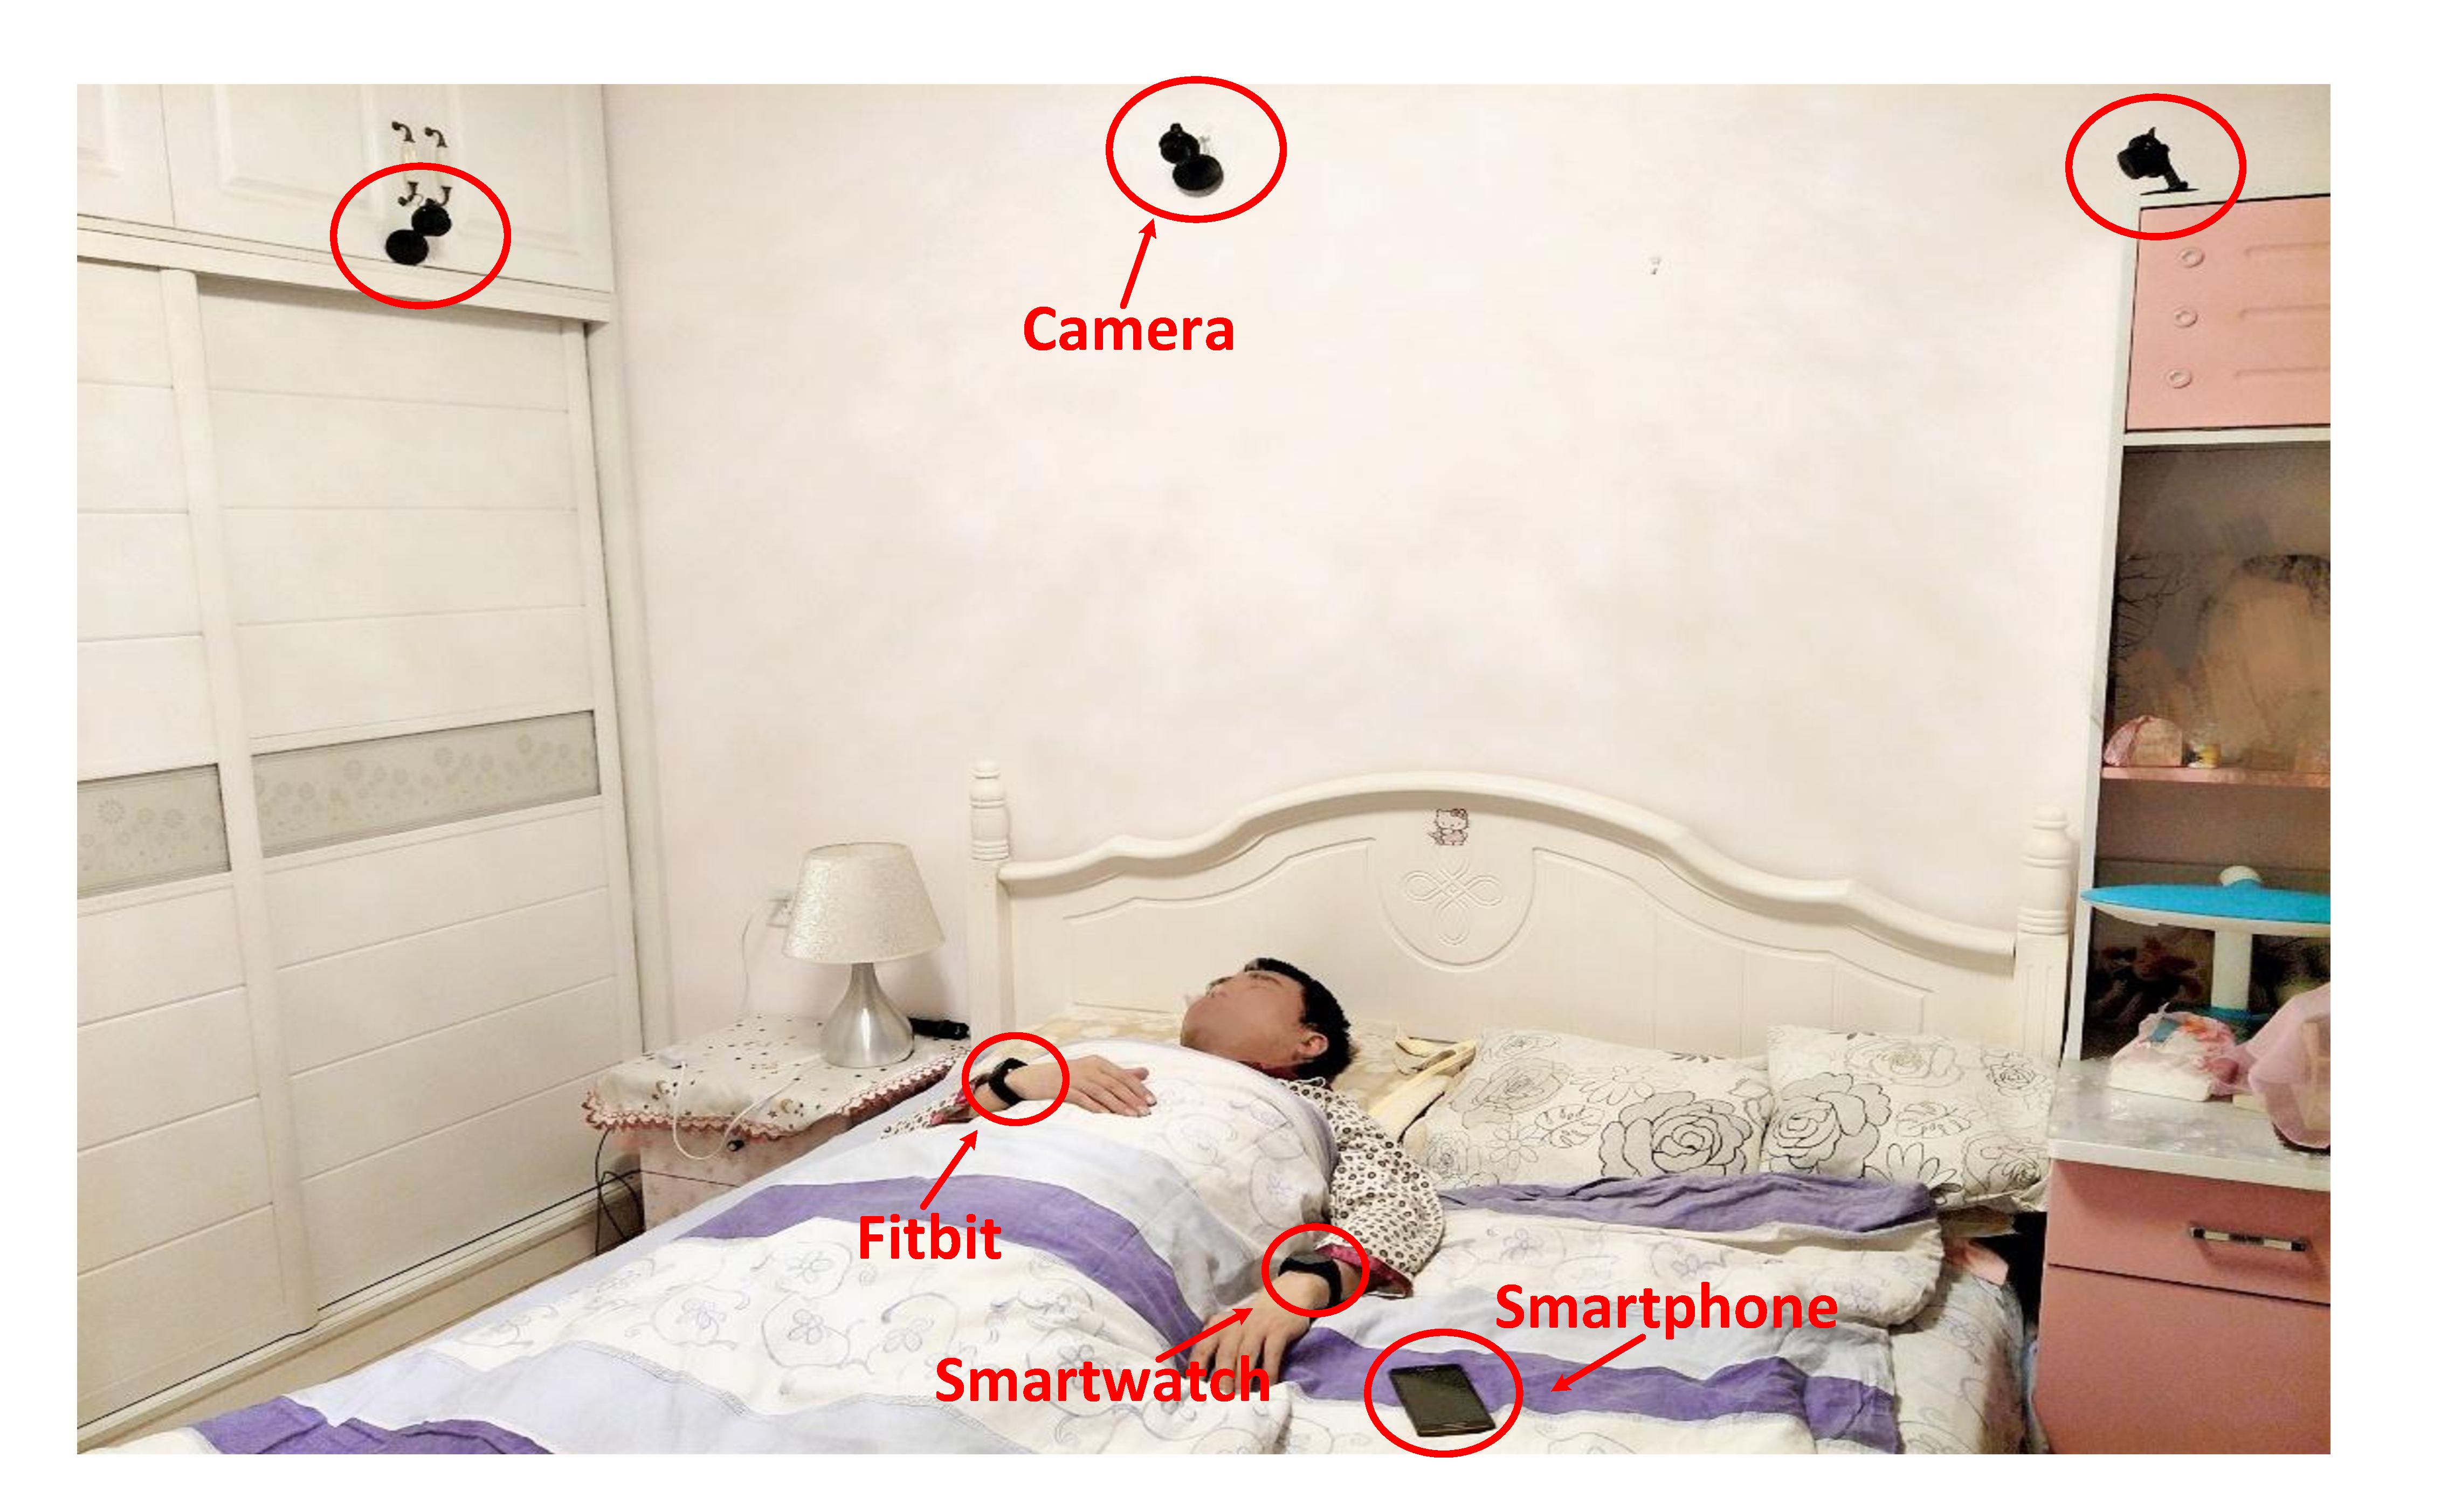
\includegraphics[width=0.52\linewidth]{Figures/setup.pdf}
	\caption{Experimental setup in one of our participants' home. }\label{fig:setup}
\end{figure}



%\section{Experimental Setup} {\systemname} is implemented on the HuaWei Smartwatch 2. The programming platform is JAVA. For simplification,
%we implement the event detection on a laptop and the collected data is processed by MATLAB. \textcolor{blue}{In our experiments, we recruit
%15 volunteers (6 males and 9 females) from 15 years old to 60 years old,  of whom 5 people are between the ages of 15 and 25, and 5 are
%between the ages of 25 and 40, and 6 people between 40 and 60 years old. According to our preliminary survey of participants, two of 40 to
%60 year old are found to have long-term sleep disorders,  one with difficulty falling asleep and having a light sleep with more dreams, and
%another participant with the symptoms of awaking at night and early awakening, and there is a 53-year-old participant have been troubled by
%snoring, they are the focus of our attention. In addition, other participants occasionally suffer some sleep problems such as insomnia,
%snore and so on.} The experiments are conducted over two weeks, and during experiments, these volunteers sleep alone in a quiet room and
%each of them sleeps at least 6 hours. Moreover, each participant is asked to wear a smartwatch and Fitbit Charge2 \cite{fitbit} on his/her
%wrist simultaneously during sleep. And the smartphone with Sleep As Android \cite{SleepAndroid} is placed beside the participant's body.
%Considering that there is no absolute ground truth to detect sleep stage and the operations of other professional medical equipment are
%complicated, we leverage the result of Fitbit Charge2, a comfortable and effortless bracelet, as the ground truth. Sleep As Android, a
%widely used app for sleep detection, run the whole sleep process for comparing with our system. At the same time, to test the reliability
%of our methods, we use the video camera to monitor the sleep, and those recorded data by camera are set as groundtruth during the
%experiment. \textcolor{red}{Fig.00000} illustrates the experimental scene for our system.



\subsection{User Participation} We have recruited 15 volunteers to participate in our experiments. Our
participants include 6 males and 9 females, whose age spans 15 to 60 years. Two of our participants have been diagnosed with long-term,
on-going sleep-related disorders, and one participant has described that his sleep is significantly affected by snoring. The rest of our
participants report their sleep quality as up and down and they could have poor sleeps from time to time.

\subsection{Experimental Setup}
After obtaining IRB approval and consents of our participants, we have conducted our experiments at 15 homes over a two-week period. We
collected \FIXME{200} sets of nocturnal sleep data from our participants. During the experiment, our volunteers slept alone in a bedroom at
home, and they slept for at least 6 hours per day.


Our participants are asked to wear a smartwatch on their wrists. Fig.~\ref{fig:setup} shows the experimental setup where we placed three
video cameras on the ceiling to monitor the user's sleep activities. The cameras have night vision and thus can record high-quality videos
at nights.  Fig.~\ref{fig:setup} shows the experimental setup where we placed three video cameras on the ceiling to monitor the user's
sleep activities. The cameras have night vision and thus can record high-quality videos at nights. We inspect the video footage to manually
label the user's sleep activities and use these as the ground truth to evaluate \systemname. We use the sleep stages reported by Fitbit
Charge2 which is proven to be accurate in monitoring user's sleep stages~\cite{}. Therefore, our participants are asked to wear two
smartwatches on their wrists: a Fitbit Charge2 that runs the Fitbit app and a Huawei Smartwatch 2 that runs \systemname.

We compare our approach against a smartphone-based sleep monitoring app named Sleep as Android~\cite{SleepAndroid}. To provide a fair
comparison, we also place a smartphone next to the user's body on the bed to collect the data for Sleep as Android.
